\section{Schaltplan}
\begin{figure}[H]
    \tikzmath{
    \offsetx1=0;\offsetx2=.7;
    \offxmotor=16;
    \offymotor=-9.5;
    \offymh = -11.5;  
    \buckxA = 12.5;
    \buckxB = 2;
    \buckxC = 2;
    \buckxD = 2;
    \buckyA = -14;
    \buckyB = -10;
    \buckyC = -12;
    \buckyD = -14;
    \platineX = 10.5;
    \platineY = -1.5;
    \relayRunter=.35;
    \platineDsiplayLinksObenX=0;
    \platineDsiplayLinksObenY=-15.5;
}

\resizebox{.99\textwidth}{!}{
\begin{circuitikz}[loops/.style={circuitikz/inductors/coils=#1}]]
    % Akkus highside
    \foreach \i in {0,2,4, 6}
        {\draw (\i,0)  to[battery, l=7S] (\i,-2);}
    \draw[very thick] (0,0) to [short,-*] ++(2,0) to [short,*-*] ++(2,0) to[short,*-*] ++(2,0);
    \draw[very thick] (0,-2) to [short,*-*] ++(2,0) to [short,*-*] ++(2,0) to[short,*-] ++(2,0);
    \draw (0+\offsetx1,-2) to[fuse, *-] (0+\offsetx1,-3.5);


    % Relay
    \draw (-.3+\offsetx1,-3.5) rectangle (.8+\offsetx1,-4.5);
    \draw (0+\offsetx1,-4.5) to[normal open switch,mirror] (0+\offsetx1,-3.5);
    \ctikzset{inductors/scale=.6, inductor=american}
    \draw (.8+\offsetx1, -4.4) -- (.55+\offsetx1,-4.4) to[L, loops=4] (.55+\offsetx1,-3.6) -- (.8+\offsetx1, -3.6);

    % Akkus lowside
    \draw (0+\offsetx1,-4.5) to[fuse, -*] (0+\offsetx1,-6);
    \foreach \i in {0,2,4, 6}
        {\draw (\i,-6)  to[battery, l=7S] (\i,-8);}
    \draw[very thick] (0,-6) to [short,*-*] ++(2,0) to [short,*-*] ++(2,0) to[short,*-*] ++(2,0);
    \draw[very thick] (0,-8) to [short,-*] ++(2,0) to [short,*-*] ++(2,0) to[short,*-*] ++(2,0);

    % Pfeile Akkus
    \draw[-latex] (6,0) -- ++(.5,0) node[right] {\scriptsize BHH};
    \draw[-latex] (6,-2) -- ++(.5,0) node[right] {\scriptsize BHL};
    \draw[-latex] (6,-8) -- ++(.5,0) node[right] {\scriptsize BLL};
    \draw[-latex] (6,-6) -- ++(.5,0) node[right] {\scriptsize BLH};

    % Notaus
    \draw (1.5+\offsetx1,-3.5) to[normal closed switch, mirror, l_=NOTAUS, -*] (1.5+\offsetx1,-2);
    \draw (1.5+\offsetx1,-3.5) to[short, -*] (1.5+\offsetx1,-3.6) -- (.8+\offsetx1,-3.6);

    % Precharge button
    % \draw (0+\offsetPrechargeX, -6) to[R, l_=10<\ohm>] (0+\offsetPrechargeX, -4) to[nopb, mirror, l={{{{\rotatebox[origin=c]{-90}{\scriptsize PRECHARGE}}}}}] (0+\offsetPrechargeX, -2);
    \draw (.8+\offsetx2, -3.6) to[nopb] (3+\offsetx2, -3.6); 
    \path (.8+\offsetx2, -3.6) -- (3+\offsetx2, -3.6) node[midway, below] {\scriptsize PRECHARGE};
    \draw (3+\offsetx2, -3.6) -- (4, -3.6) to[R, l=10<\ohm>, -*] (4,-6);
  

    % Minus relay auf platine
    %\draw (.8+\offsetx1, -4.4) -- (4,-4.4);
    %\draw (4.4,-4.4) -- (6,-4.4);
    \draw (.8+\offsetx1, -4.4) -- (1,-4.4);
    \draw[-latex reversed] (1,-4.4) -- ++(.2,0) node[right=-.1] {\scriptsize A2};

    %%--------------------------------------------------------------%%

    % Motorregler, Motor
    \foreach \x/\y/\ii in {\offxmotor/\offymotor/1, \offxmotor/\offymh/2}{
        \draw (\x, \y-.25) -- (\x-1.5,\y-.25);
        \draw (\x, \y) -- (\x-1.5,\y);
        \draw (\x, \y+.25) -- (\x-1.5,\y+.25);
        \draw (\x, \y) node[very thick, circle, draw, minimum size=3, fill=white] {A200};

        %\draw[thick] (\offxmotor-4, \offymotor-.5) rectangle (\offxmotor-1.5, \offymotor+.5);
        \node[thick, draw, fit={(\x-4, \y-.8) (\x-1.5, \y+.8)},inner sep=0, align=center] {\scriptsize Master SPIN 220 PRO OPTO};

        \draw[-latex reversed, thick] (\x-4, \y-.6) -- ++(-.65,0) node[left] {\scriptsize BLL};
        \draw[-latex reversed, thick] (\x-4, \y+.6) -- ++(-.65,0) node[left] {\scriptsize BHH};
        \draw[-latex reversed] (\x-4, \y+.2) -- ++(-.4,0) node[left] {\scriptsize PWM-M\ii};
        \draw[-latex] (\x-4, \y-.2) -- ++(-.4,0) node[left] {\scriptsize Serial-M\ii};
    }

    % Buck converter
    ctikzset{inductors/scale=.4, inductor=american}
    \foreach \x/\y in {\buckxA/\buckyA, \buckxB/\buckyB, \buckxC/\buckyC, \buckxD/\buckyD}{
        \node[thick, draw, fit={(\x, \y+.55) (\x+2.5, \y-.55)},inner sep=0, align=center] {{{{\scriptsize DC/DC}}}};

        \draw (\x-1.25,\y+1-\relayRunter) to[normal open switch] ++(.5,0) --++(.25,0) -- ++(0.35,0) -- (\x-.15,\y+.4) -- (\x,\y+.4) node[right=-.1] {\tiny VIN+};

        \draw (\x-1.35, \y+1.3-\relayRunter) rectangle (\x-.4, \y+.5-\relayRunter);

        \draw (\x-1.25, \y+.4-\relayRunter) -- (\x-1.25, \y+.6-\relayRunter) to[L, loops=4] (\x-.5,\y+.6-\relayRunter) -- (\x-.5,\y+.4-\relayRunter) to[short, -*] (\x-.5,\y-.4);

        \draw[-latex reversed] (\x-1.25, \y+.4-\relayRunter) -- (\x-1.5, \y+.4-\relayRunter) node[left] {\tiny BHL};

        
        \draw[-latex reversed] (\x, \y-.4) node[right=-.1] {\tiny VIN-} -- ++(-1.75,0) node[left] {\scriptsize BLL};
        \draw[-latex reversed] (\x-1.25, \y+1-\relayRunter) -- ++(-.5,0) node[left] {\scriptsize BHH};
    }

    \draw[-latex] (\buckxA+2.5, \buckyA+.4) node[left=-.1] {\tiny VOUT+} -- ++(.5,0) node[right]{\scriptsize CAN-VCC};
    \draw[-latex] (\buckxA+2.5, \buckyA-.4) node[left=-.1] {\tiny VOUT-} -- ++(.5,0) node[right]{\scriptsize CAN-GND};
    %\draw[fill] (\buckxA+3, \buckyA-.5) rectangle (\buckxA+3.1, \buckyA+.5);
    %\draw[double, -latex] (\buckxA+3.1, \buckyA) -- ++ (.5,0) node[right] {\small CAN-Bus};

    \foreach \x/\y/\ii in {\buckxB/\buckyB/1, \buckxC/\buckyC/2, \buckxD/\buckyD/3}{
        \draw (\x+2.5, \y+.4) node[left=-.1] {\tiny VOUT+} -- ++(2,0);
        \draw (\x+2.5, \y-.4) node[left=-.1] {\tiny VOUT-} -- ++(2,0);
        
        \node[thick, draw, fit={(\x+4.5, \y+.55) (\x+6.5, \y-.55)},inner sep=0, align=center] {{{{\scriptsize SERVO}}}};
        \draw(\x+4.5, \y+.4) node[right=-.1] {\tiny VCC};
        \draw(\x+4.5, \y-.4) node[right=-.1] {\tiny GND};
        \draw[-latex reversed] (\x+4.5, \y) node[right=-.1] {\tiny D} -- ++(-.5,0) node[left] {\tiny PWM-S\ii};

        \draw[thick] (\x+6.3, \y) circle (.07);
        \draw (\x+6.3, \y+.12) arc (90:270:.12);
        \draw (\x+6.8, \y+.05) arc (90:-90:.05);
        \draw[fill] (\x+6.8, \y) circle (.025);
        \draw (\x+6.3 , \y+.12) -- (\x+6.8, \y+.05);
        \draw (\x+6.3 , \y-.12) -- (\x+6.8, \y-.05);
    }

    %% Ansteuerungs-Platine Relay
    \draw[very thick] (\platineX, \platineY) rectangle (\platineX+5, \platineY-5);
    \node[thick, fit={(\platineX+1, \platineY) (\platineX+5, \platineY-5)},inner sep=0, align=center] {\small Platine\\Relaisansteuerung\\ siehe \autoref{fig:plat:relais}};

    \foreach \y/\text in {.5/7, 2/6, 3.5/8}{
        \draw (\platineX, \platineY-\y) -- ++(.5,0) -- ++(0,-1) -- ++(-.5,0);
        \draw (\platineX, \platineY-.25-\y) to[short, -*] ++(.25,0);
        \draw (\platineX, \platineY-.75-\y) to[short, -*] ++(.25,0);
        \draw (\platineX+.5, \platineY-.5-\y) node[right] {\small J\text};
    }

    \draw[-latex reversed] (\platineX, \platineY-.75) -- ++(-.5,0) node[left] {\scriptsize BHL};
    \draw[-latex reversed] (\platineX, \platineY-1.25) -- ++(-.5,0) node[left] {\scriptsize BLL};

    \draw[-latex] (\platineX, \platineY-2.25) -- ++(-.5,0) node[left] {\scriptsize A2};
    \draw[-latex reversed] (\platineX, \platineY-2.75) -- ++(-.5,0) node[left] {\scriptsize BLL};
    
    \draw[-latex reversed] (\platineX, \platineY-3.75) -- ++(-.5,0) node[left] {\scriptsize BLH};
    \draw[-latex reversed] (\platineX, \platineY-4.25) -- ++(-.5,0) node[left] {\scriptsize BLL};

\end{circuitikz}
}

    \caption{Schaltplan Leistungselektronik\label{fig:schaltLeistung}}
\end{figure}
Für die Verbindung zwischen Board- und Leistungselektronik siehe \autoref{fig:schaltBoard}.

\clearpage
\section{Verkabelung}
Da wir mit beiden Motoren einen Strom von 400A haben, verwenden wir Kupferschienen zur Verteilung dieses Stromes.\\
Die Akkus gehen jeweils mit beiden Anschlüssen über einen 10mm\textsuperscript{2}-Draht auf eine Kupferschiene. Die Motorregler sind ebenfalls mit jeweils 2 10mm\textsuperscript{2}-Drähten angeschlossen, um bei diesen hohen Strömen möglichst wenig Spannungsabfall zu haben.\\
Das Hauptrelais ist über die Schmelzsicherungen direkt mit den Kupferschienen verschraubt.
\begin{figure}[H]
    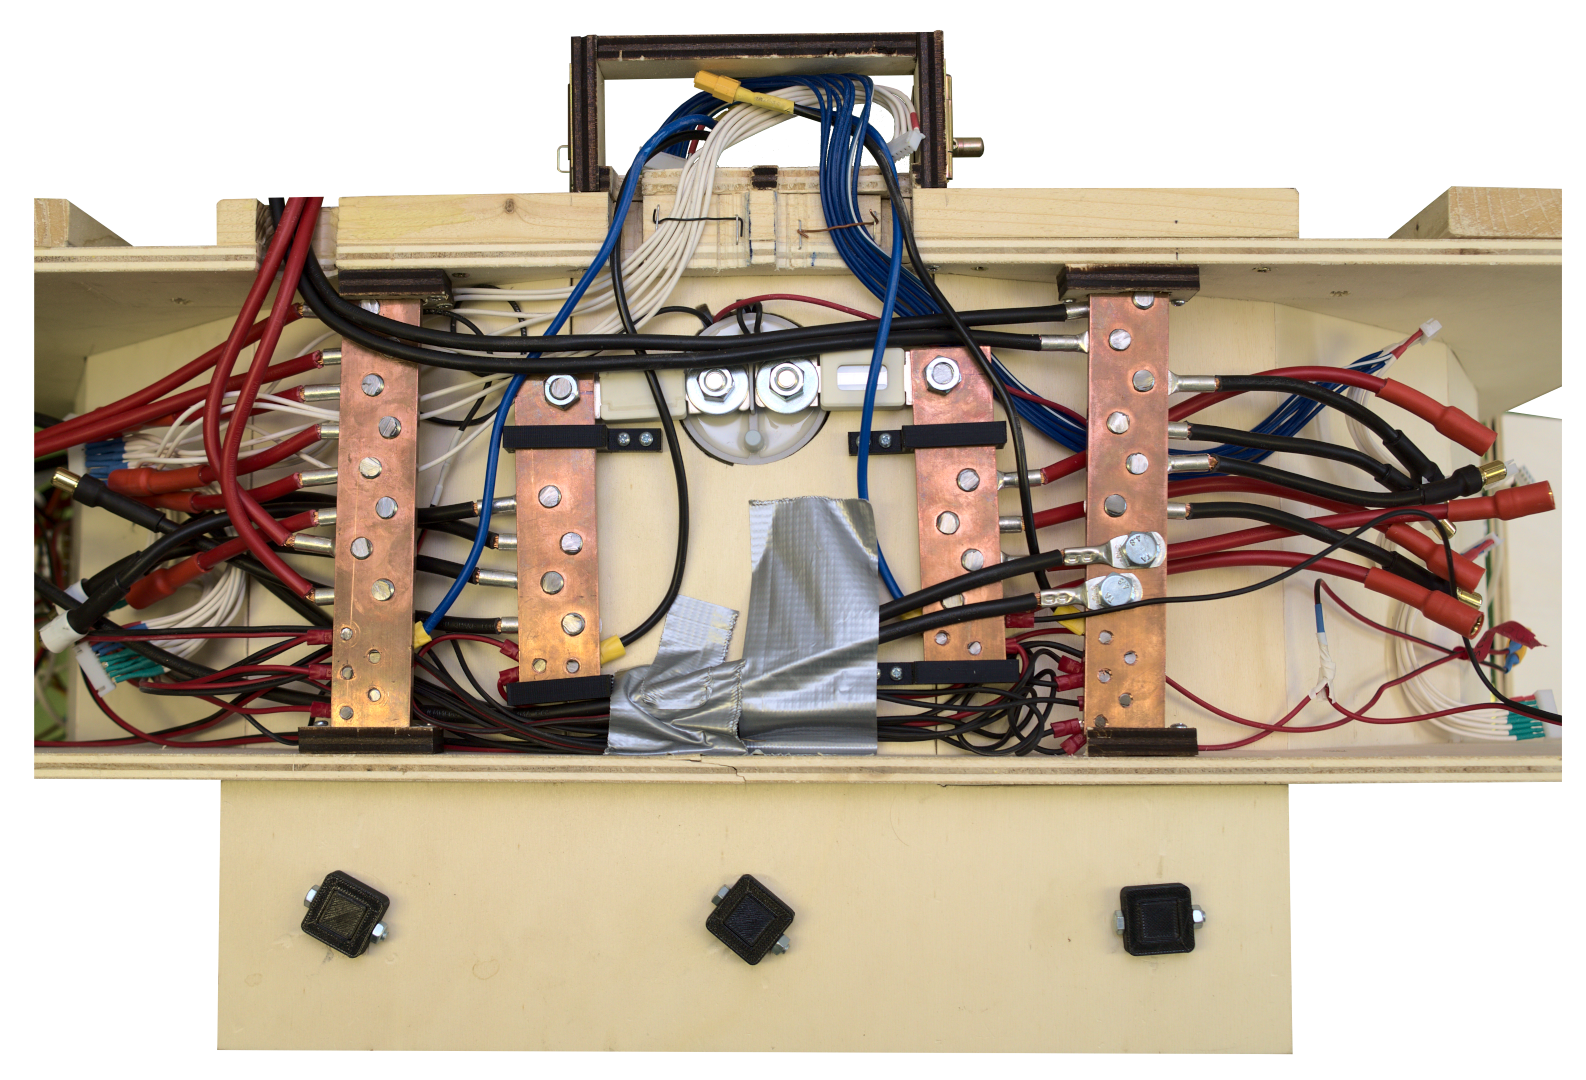
\includegraphics[width=.99\textwidth]{Fotos/Konstruktion/DSC_8836.png}
    \caption{Verkabelung Kupferschienen}
\end{figure}


\clearpage